\documentclass[a4paper, 12pt]{article}
\usepackage[utf8]{inputenc}
\usepackage[russian]{babel}
\usepackage{geometry}
\usepackage{graphicx}
\usepackage{hyperref}
\usepackage{enumitem}
\usepackage{titlesec}

\geometry{left=2cm, right=1.5cm, top=2cm, bottom=2cm}
\hypersetup{colorlinks=true, linkcolor=blue, filecolor=magenta, urlcolor=cyan}
\titleformat{\section}{\normalfont\Large\bfseries}{\thesection}{1em}{}

\title{Руководство по выполнению ДЗ №2 по САПР \\ \large{Проектирование двухсторонней печатной платы}}
\author{Создано админом группы Р3331, для ВТ}
\date{\today}

\begin{document}

\maketitle
\tableofcontents

\newpage
\section{Цель работы}
Спроектировать двухстороннюю печатную плату (ПП) с заданными параметрами в соответствии с вариантом.

\section{Исходные данные}
\subsection{Структура задания}
\begin{itemize}
	\item Каждому студенту выдаётся лист формата А4 с индивидуальными параметрами:
	      \begin{itemize}
		      \item Количество модулей (микросхем): M (например, 19)
		      \item Количество цепей: K (например, 39)
		      \item Контакты на модуле (микросхем): N (например, 14)
		      \item Запрещённые выводы: заданы индивидуально (например, 7, 14 — подключены к питанию)
	      \end{itemize}
	\item Формат описания цепей:
	      \begin{verbatim}
    Цепь #Ki модуль/контакт, модуль/контакт, ...

    Пример:
    Цепь #1 14/2, 1/8, 18/10, 11/8, 19/4
    \end{verbatim}

	      Простым языком - каждая такая цепь описывает соединение определённых контактов определённых модулей.
	      В данном случае, соединяются модули (микросхемы) с номерами 14, 1, 18, 11, 19 через контакты 2, 8, 10, 8, 4.

	\item Строка подключения к разъёму:
	      \begin{verbatim}
    На разъём: 37, 10, 7, 25, 3, 39, 22, 16, 35, 36
    \end{verbatim}

	      Представьте что это просто какой-то выходной разъём, или ещё лучше - торчащие из платы пины.
	      Например, вот из платы торчат какие-то пины, и часть из них может использоваться для протокола jtag, другая часть ещё для чего-то и т.п. Нам это в рамках этого дз неважно.

	      \begin{figure}[h!]
		      \centering
		      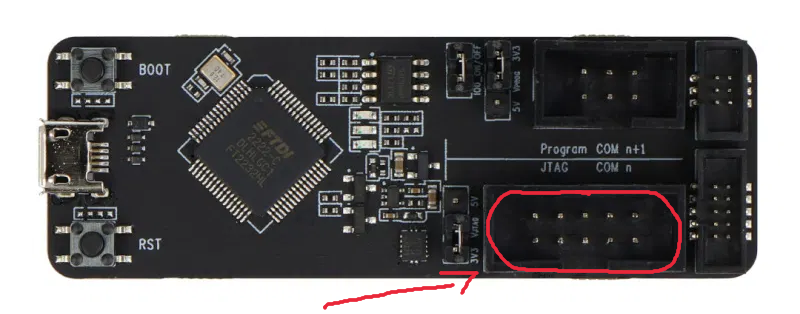
\includegraphics[width=0.62\textwidth]{docs/pinout.png}
		      \caption{Пример разъёма на плате}
	      \end{figure}
\end{itemize}

\subsection{Обозначения}
\begin{itemize}
	\item Микросхемы: U1, U2, ..., UM (это произвольные микросхемы с N контактов)
	\item Разъём для внешних цепей: J2 (индекс 2 для примера. Просто надо обозначить выходной разъём)
	\item Запрещённые контакты: не участвуют в соединениях (gnd, vcc)
\end{itemize}

\subsection{Пример варианта}
\begin{figure}[h!]
	\centering
	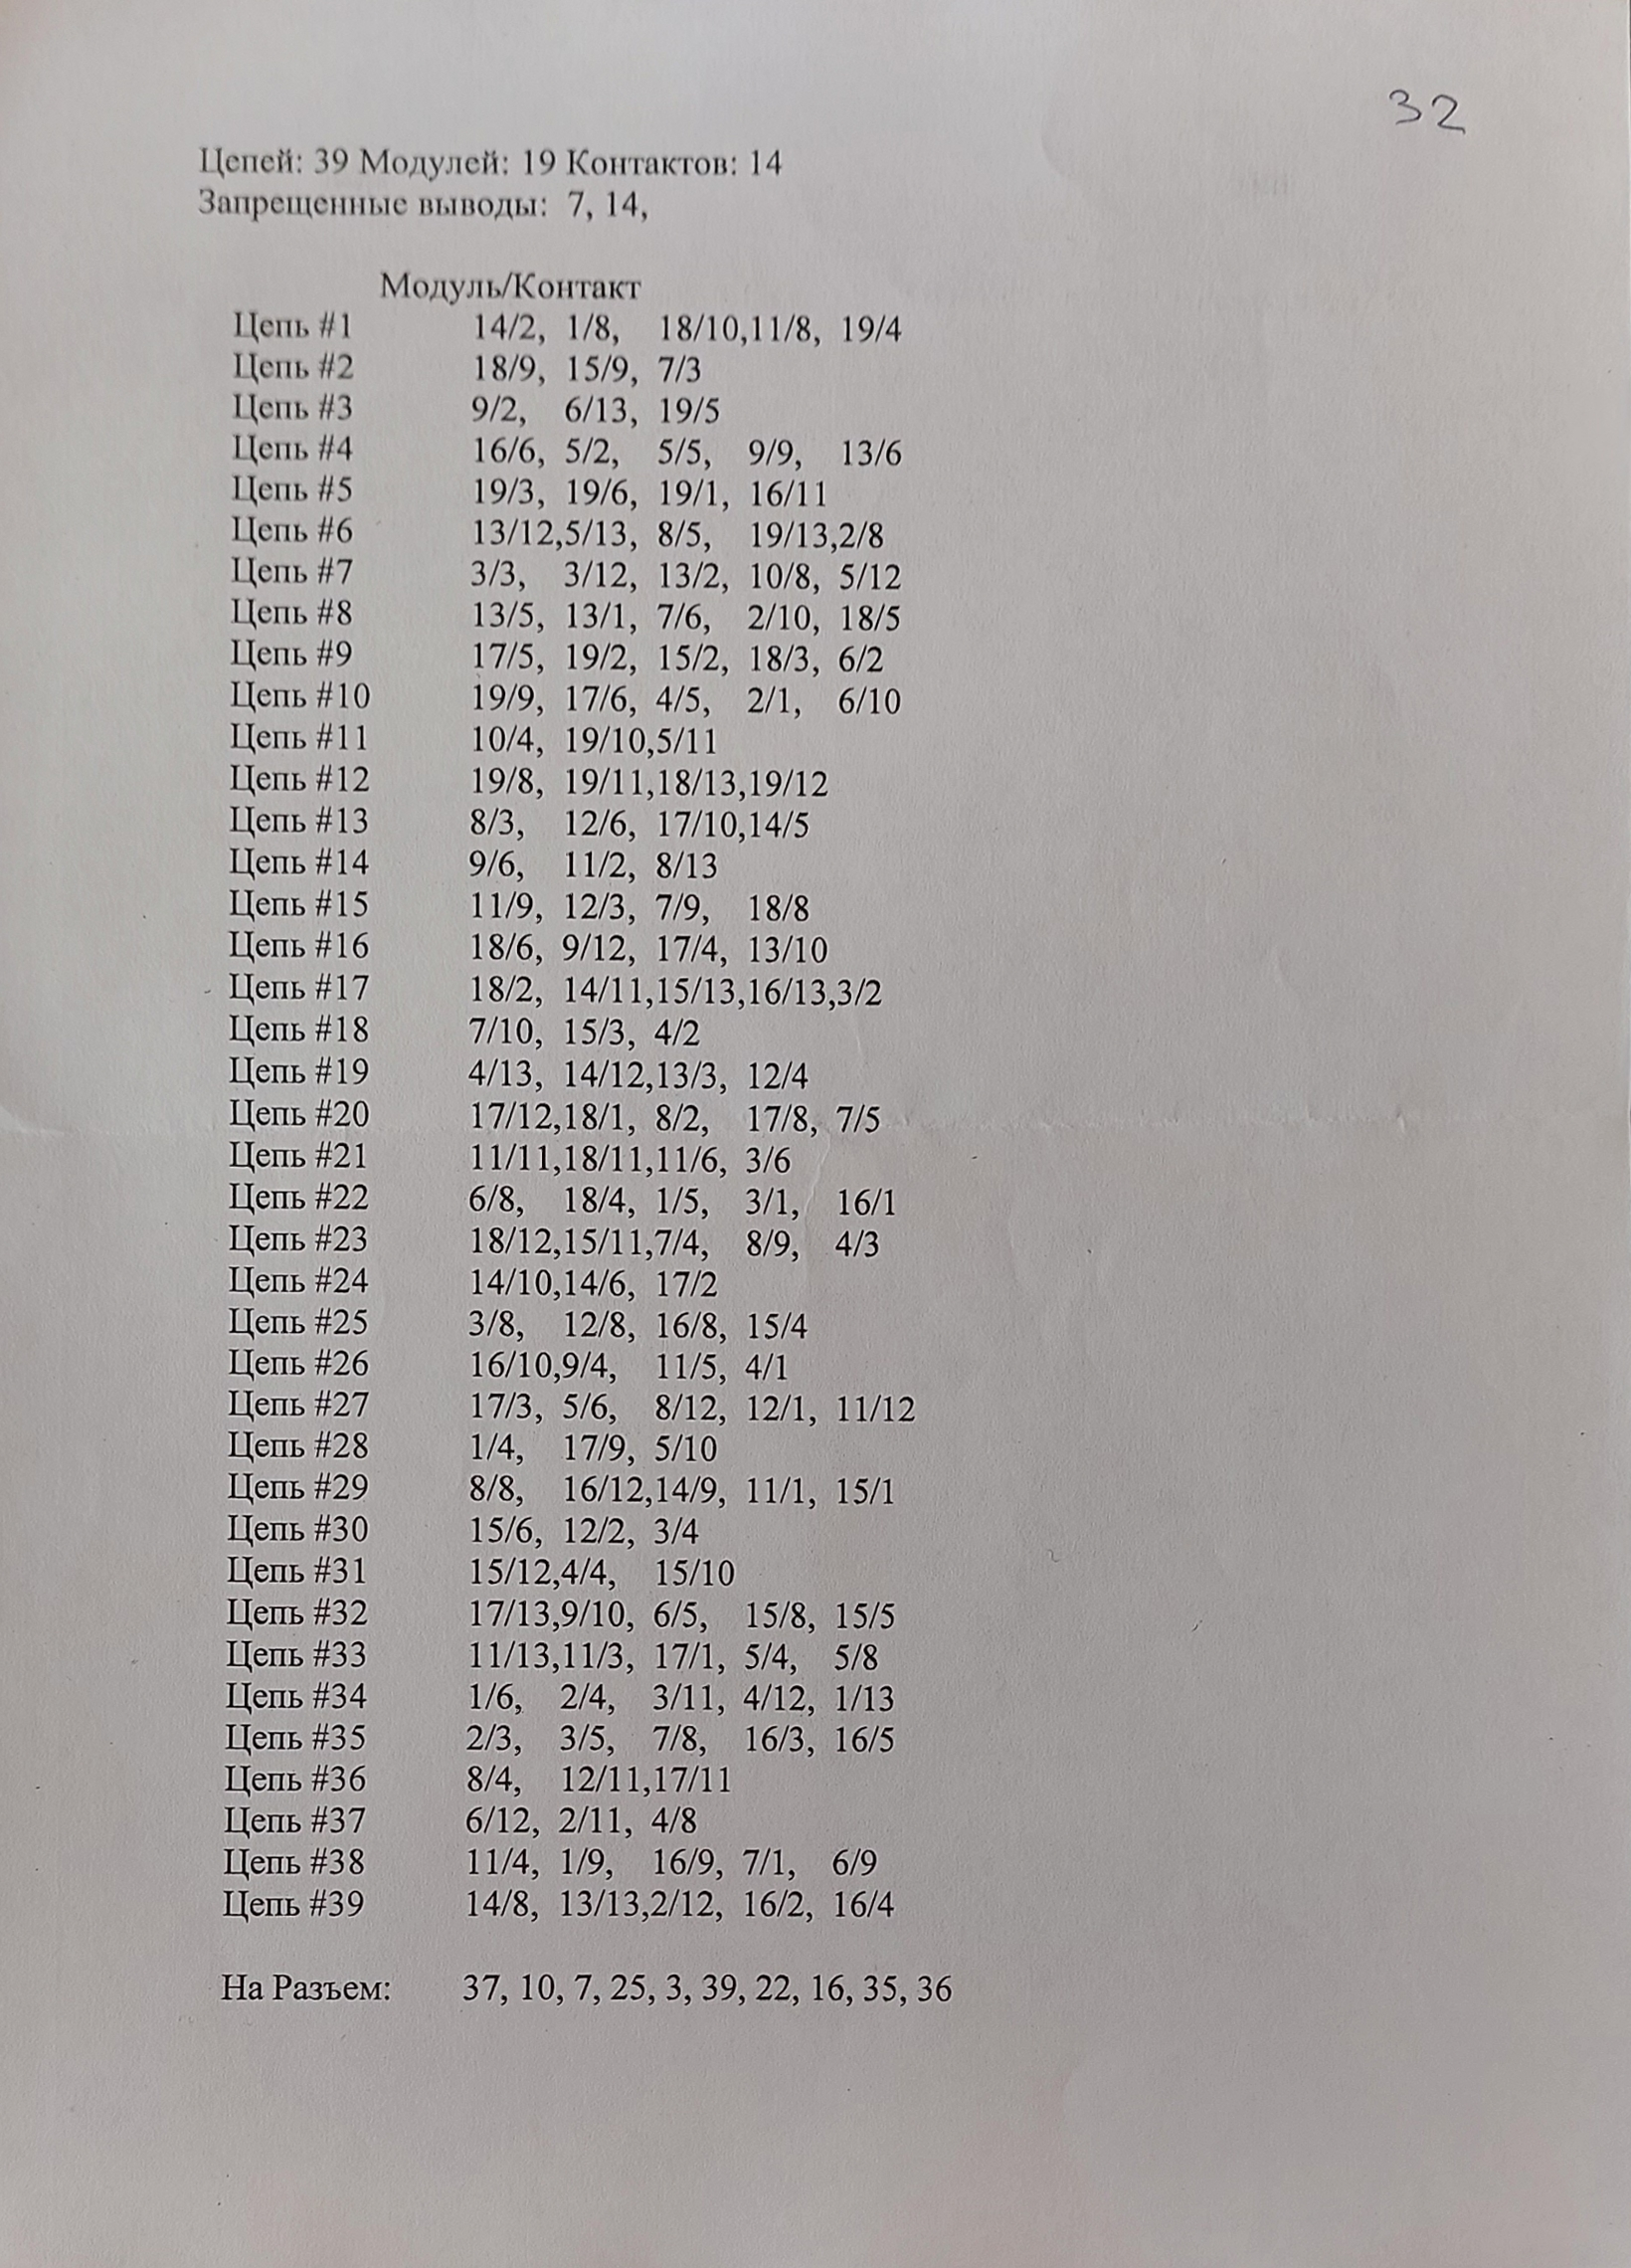
\includegraphics[width=0.76\textwidth]{docs/hw_ex.jpg}
	\caption{Мой варик - 32й}
\end{figure}

\section{Этапы выполнения}
\subsection{Пререквизиты}
\textbf{Я сделал шаблон (hw2\_template), взять его можно в} \underline{\textbf{\href{https://github.com/Imtjl/ic-pcb-engineering/tree/master/hw2}{репозитории}}}

\subsection{Подготовка схемы}
\begin{enumerate}
	\item Разместить 14-контактные микросхемы (например, DIP-14) на плате
	\item Разместить разъём J2 (например, формата JST) на выделенное количество цепей + питание (VCC), земля (GND)
	\item Создать схему соединений на основе списка цепей.
	\item Отметить запрещённые контакты (например, 7 и 14) как подключённые к шинам питания.
	\item Цепи, указанные в строке «На разъём», вывести на контакты J2.
\end{enumerate}

\subsection{Трассировка ПП}
\begin{itemize}
	\item Использовать двухстороннюю компоновку.
	\item Минимизировать пересечения дорожек.
	\item Учесть требования к ширине проводников и зазорам (выберите фиксированную сетку, не мельчите и норм).
\end{itemize}

\subsection{3. Проверка (DRC)}
Выполнить Design Rule Check в выбранном ПО (например, KiCad, Altium):
\begin{itemize}
	\item Отсутствие коротких замыканий.
	\item Корректность подключения цепей к разъёму.
	\item Изоляция запрещённых контактов.
\end{itemize}

\section{Пример оформления}
\subsection{Исходные данные студента}
\begin{itemize}
	\item M = 19 модулей (U1–U19)
	\item N = 14 контактов на модуле
	\item Запрещённые контакты: 7, 14
	\item Цепи: 39 (примеры см. в разделе 2.1)
	\item На разъём: цепи 37, 10, 7, 25, 3, 39, 22, 16, 35, 36
\end{itemize}

\newpage
\subsection{Визуализация цепи \#1}
\begin{verbatim}
Цепь #1: U14/2 — U1/8 — U18/10 — U11/8 — U19/4
\end{verbatim}

\begin{figure}[h!]
	\centering
	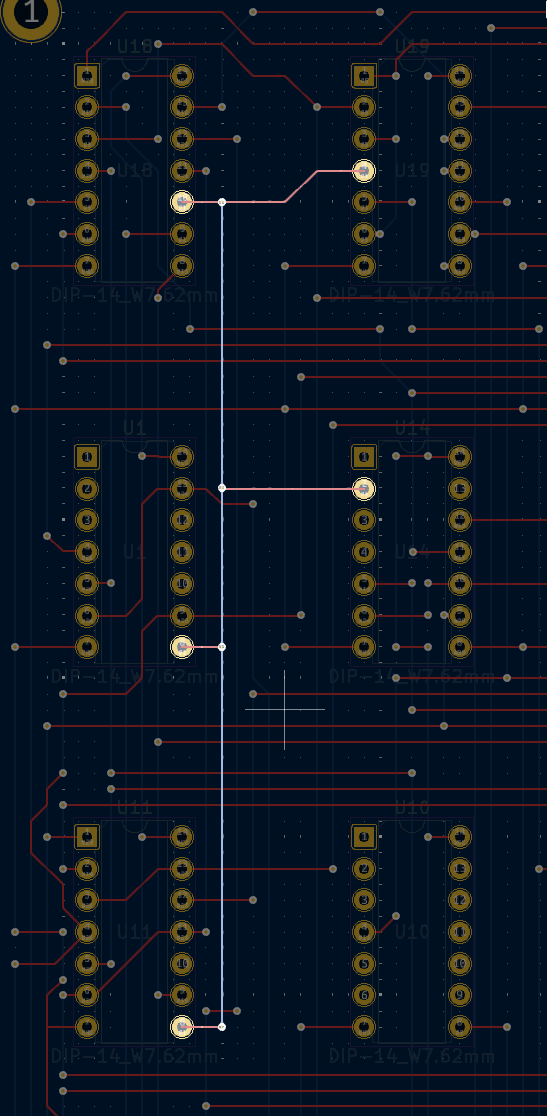
\includegraphics[width=0.5\textwidth]{docs/net1.png}
	\caption{Пример трассировки цепи}
\end{figure}

P.S. Совет: Создавайте так называемые \textbf{net} при проектировании \textbf{pcb} в KiCad. Таким образом вы сильно упростите себе жизнь (он будет подсказывать какие дорожки не заняты, подписывать каждое соединение своим номером, автоматически трассировать между ними путь и т.п.)

\section{Пример выполненных дз}

\subsection{Пример 1}
\begin{figure}[h!]
	\centering
	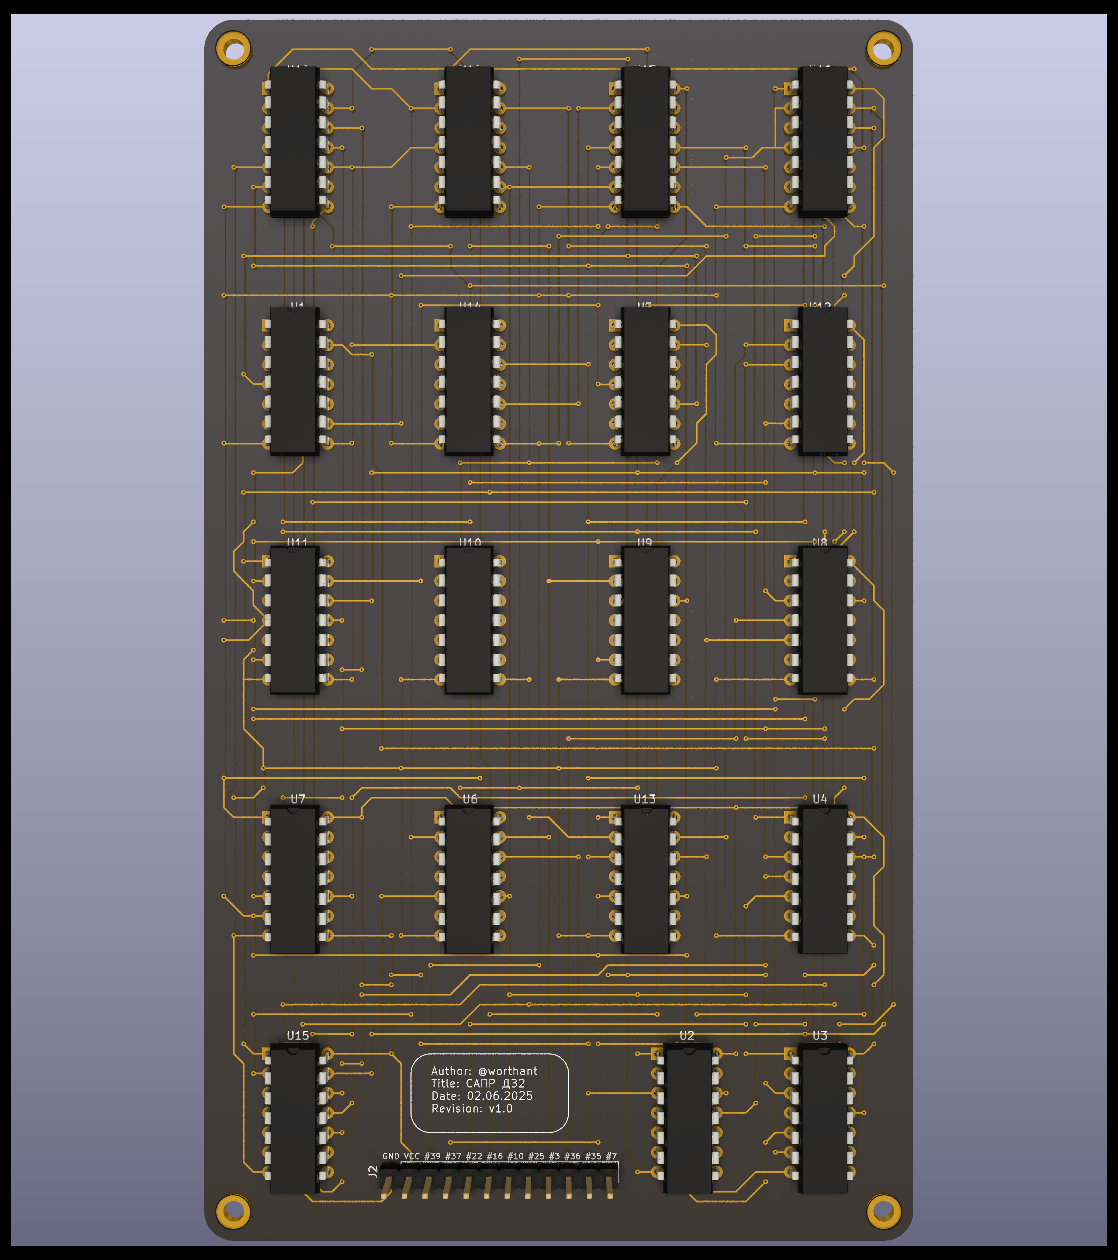
\includegraphics[width=0.9\textwidth]{docs/myhw3.png}
	\caption{Моя домашка, выполненная в KiCad 8}
\end{figure}

\newpage
\begin{figure}[h!]
	\centering
	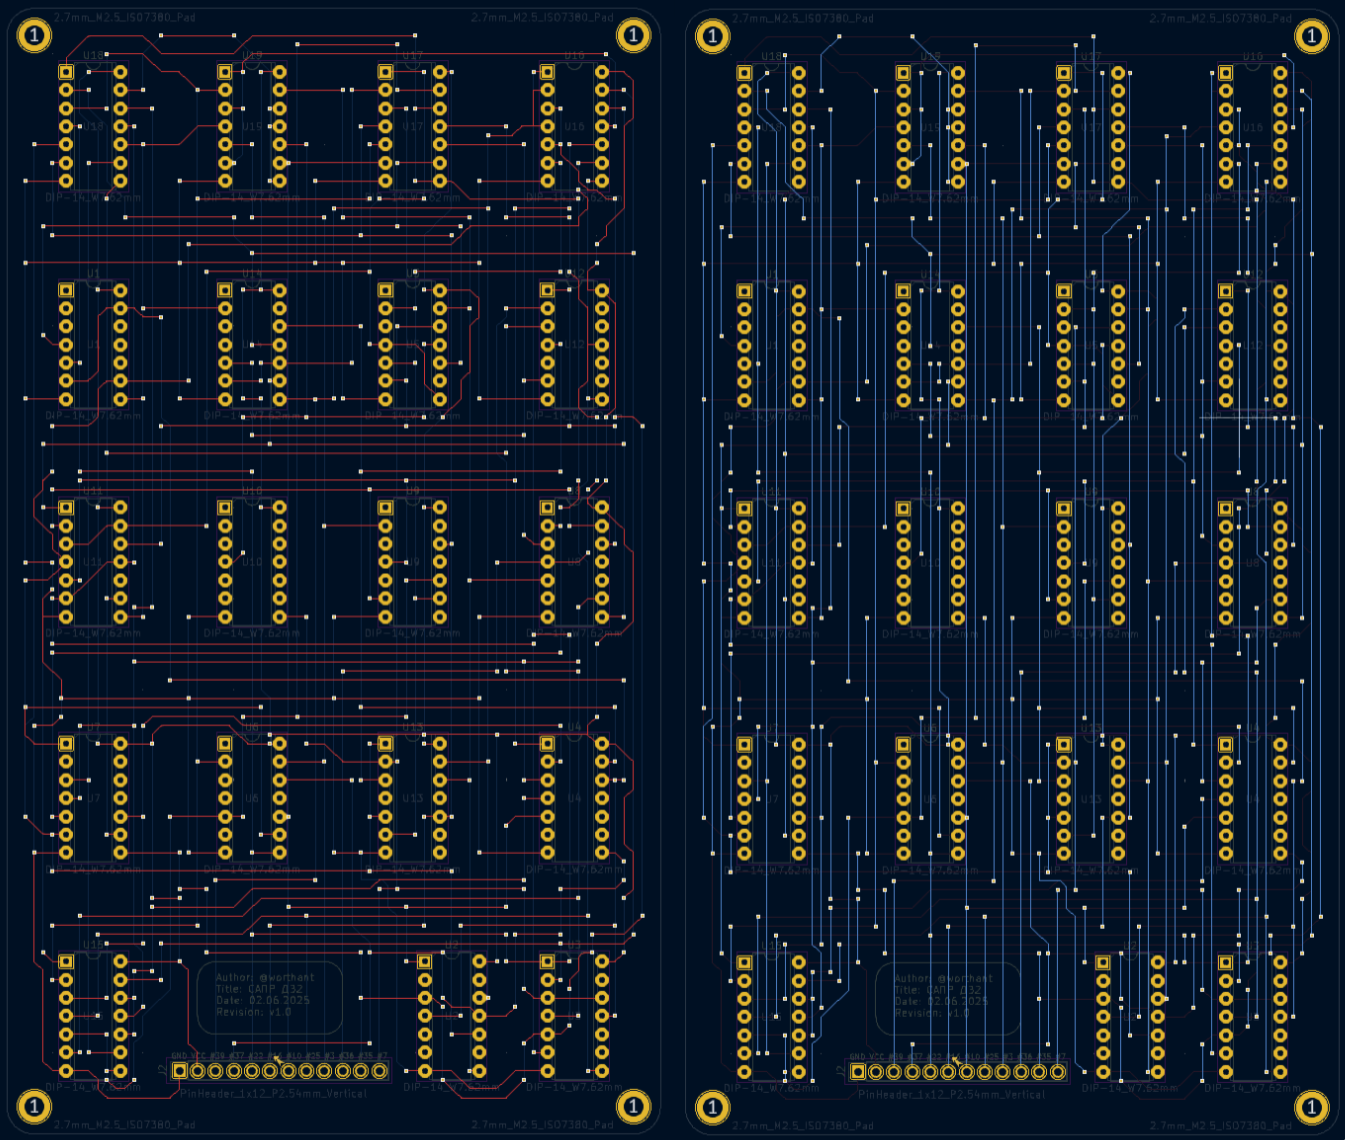
\includegraphics[width=0.9\textwidth]{docs/myhw2.png}
	\caption{Моя домашка, выполненная в KiCad 8}
\end{figure}

\newpage
\subsection{Пример 2}
\begin{figure}[h!]
	\centering
	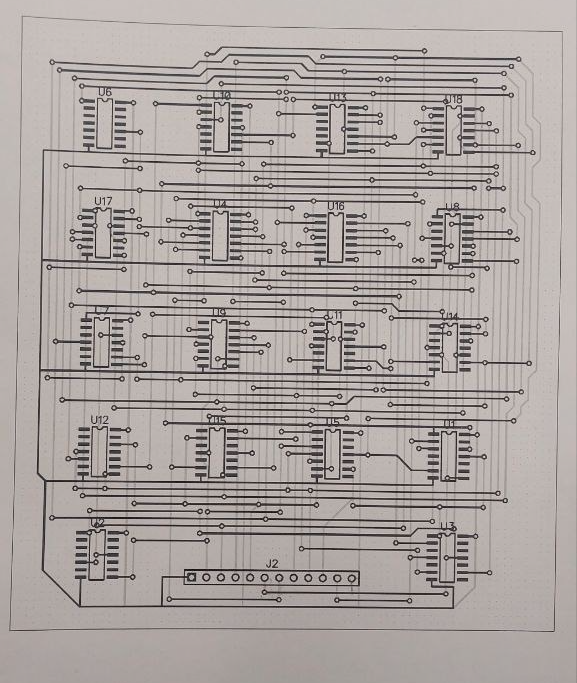
\includegraphics[width=0.9\textwidth]{docs/ex1.png}
	\caption{Есть только одна сторона. Догадаться об обратной можно по серым соединениям.}
\end{figure}

\newpage
\subsection{Пример 3}
\begin{figure}[h!]
	\centering
	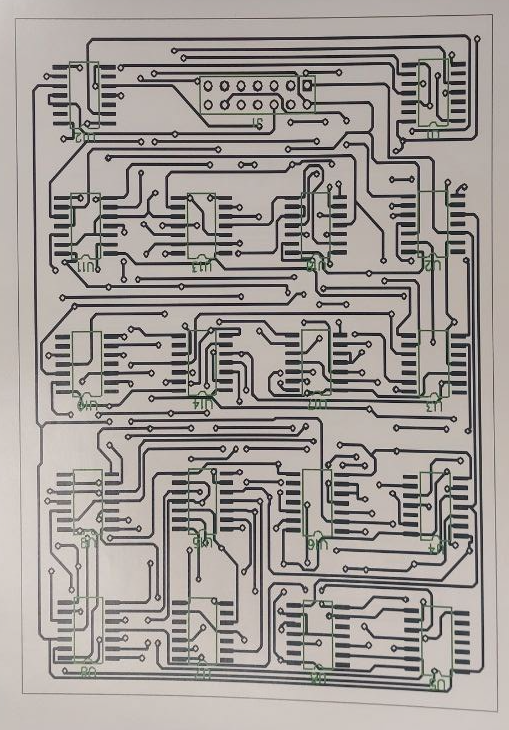
\includegraphics[angle=180,origin=c,width=0.9\textwidth]{docs/ex2.png}
	\caption{Лицевая сторона}
\end{figure}

\begin{figure}[h!]
	\centering
	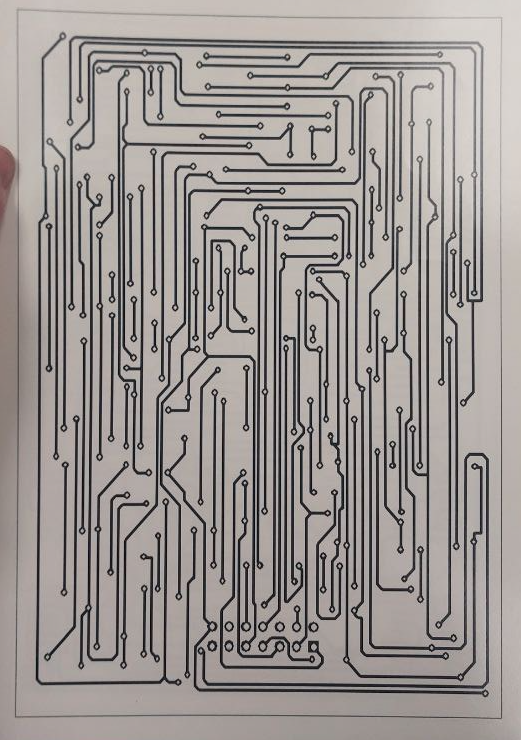
\includegraphics[width=0.9\textwidth]{docs/ex3.png}
	\caption{Обратная сторона}
\end{figure}

\end{document}
